\chapter{A Random Access Scheme based on Gain Division Multiple Access}
\label{c:rach_gdma}

Recently, random access protocol has not only caused the rise of satellite communication, but also caused the application of Internet of things (IOT) and machine to machine. In this chapter, we will implement a random access scheme based on gain division multiple access. Assumed that the system is UL transmission, and numerous devices use the same channel resources to transfer in a common evolved NodeB (eNB). Unlike ordinary random access, when a packet collision occurs, the eNB does not directly feedback HARQ (hybrid automatic repeat request), but multiuser detection (MUD) using the concept of GDMA. Then, we will introduce RACH and Grant to discuss various situations in our system further. In the second section, we will present the RA system more clearly and derive the ALOHA system's throughput. In the third section, we will introduce the random access orthogonal-frequency division multiplexing gain division multiple access (RA-OFDM-GDMA) system. Discuss the different cases of the MUD based on the variation of RACH and Grant. Then, add a preamble sequence to execute synchronization and hybrid channel gain estimation.


\section{Introduction of RACH and Grant}

RACH stands for Random access channel, which is the first message from UE to eNB when power on it. RACH is used in many places, e.g., achieve uplink synchronization between user equipment(UE) and eNB, obtain the resource for RRC connection request, etc. From the perspective of eNB, the UE signal is almost in a random fashion, e.g., casual time, random frequency, arbitrary identification. 

Before UE decides to send RACH signals (RACH preamble), many preconditions are called “Power-On to PRACH”. The steps of power-on to PRACH are described as :

\begin{enumerate}[leftmargin=\leftmargin+\widthof{Prefix}]
\item[Step 1)] UE is off.
\item[Step 2)] Power On UE.
\item[Step 3)] UE tune to a specific frequency.
\item[Step 4)] Time and Frame synchronization (PSS SSS decode).
\item[Step 5)] Physical Cell ID(PCI) , PBCH detection.
\item[Step 6)] Initial RACH process.
\end{enumerate}

, where Primary Sync Sequence(PSS) provides Radio Frame Boundary using preamble sequence and Secondary Sync Sequence (SSS) provides Subframe Boundary using correlation windows.

There are two type of RACH process : contention-based and contention-free. 

The steps of Contention-base RACH in 5G NR are summarized below.
\begin{enumerate}[leftmargin=\leftmargin+\widthof{Prefix}]
\item[Step 1)] Preamble transmission : The preamble is assigned by the UE. The UE selects one of the 64 preambles from the system information provided by the eNB to compete (Msg1).
\item[Step 2)]Random Access Request : If a collision occurs, perform a back of. If successful, the eNB knows the UE information.
\item[Step 3)]Radio Resource Control Connection Request : Reply Random Access response to UE, including Timing Advance and UL grant.
\item[Step 4)] RRC Connection Setup : After receiving the RAR, the UE will upload the ID with the UE information in the UL grant. If no other UE uses the same preamble in Msg1, the UE will compete for the channel resources of the RAP.
\end{enumerate}


The steps of Contention-free are summarized below.
\begin{enumerate}[leftmargin=\leftmargin+\widthof{Prefix}]
\item[Step 1)] Preamble Allocation : The preamble is assigned by the eNB.
\item[Step 2)] Preamble Transmission : The eNB knows the UE information.
\item[Step 3)] 5)	Radio Resource Control Connection Request : Reply Random Access response to UE, including Timing Advance and UL grant.
\end{enumerate}

\begin{figure}[t!]
 \centering
 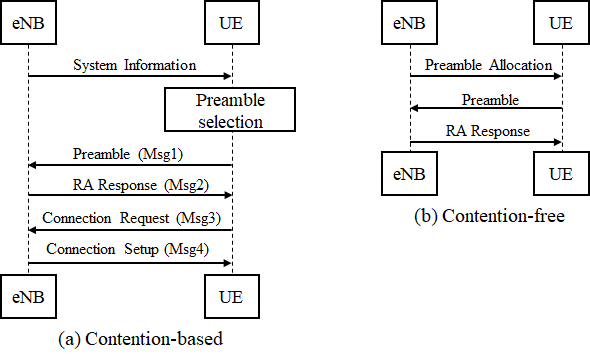
\includegraphics[width=10cm]{fig/RACH_contention_based_free.png}
 \caption{Two type of RACH process.}
 \label{fig:RACH_contention}
\end{figure}

The paper\cite{shahab2019grant} classified that RACH-based Grant-base, RACH-based Grant-free, RACH-free Grant-free system, where Grant means whether the number of users choosing a particular frequency sub-band is random. Users transmit data on an “arrive and go” basis (grant-free), or the receiver already allocates some specific number of users a particular subband. The transmission is scheduling(grant-based), e.g., users are aligned/connected in typical cellular communication.

\section{Introduction of Random Access System}

\begin{figure}[b!]
 \centering
 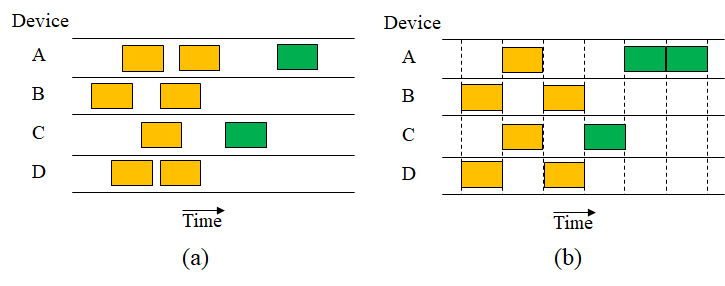
\includegraphics[width=10cm]{fig/RACH_slotted_unslotted.png}
 \caption{(a) An unslotted ALOHA system. (b) A slotted ALOHA system.}
 \label{fig:RACH_slotted_unslotted}
\end{figure}

\begin{figure}[t!]
 \centering
 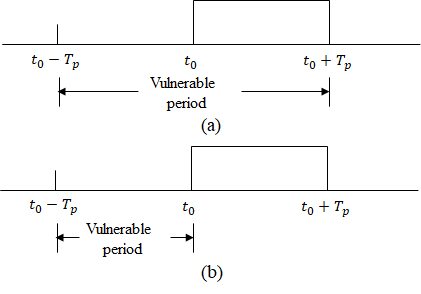
\includegraphics[width=10cm]{fig/RACH_vulnerable.png}
 \caption{(a) The vulnerable period for unslotted system. (b) The vulnerable period for slotted system.}
 \label{fig:RACH_vulnerable}
\end{figure}

In this section, we consider a multiuser communication system in which users transmit information in packets with common channel resource. In contrast to the CDMA or TDMA, the transmission would not be scheduled in advance. In conventional MA, the channel resource would be wasted during the period that device is granted to access, but it has nothing to say. If the number of device is massive, these MA will waste more resources. However, this is just a situation where random access techniques tend to become efficient. The access methods described below are basically random because packets are generated according to some statistical models. Users access the channel when they have one or more packets overlap in time, they collide, and, hence, a conflict results. If more than one frame are transmitted, they interfere with each other and are lost. If ACK not received within the timeout, then a user picks random backoff time. An ALOHA scheme \cite{abramson1970aloha} was originally analyzed for random access system at the University of Hawaii in 1970, which provides access to a common communication channel from multiple independent packet transmitters by the simplest of all mechanisms. The ALOHA system can be classified into two types in fig by slotted(RACH).\ref{fig:RACH_slotted_unslotted}.

We assume that the start time of packets that are transmitted is a Poisson point process having an average rate of $\lambda$ packets/s at the receiver.
Let $T_s$ denote the time duration of a packet. Then, the normalized channel traffic $G$, is defined as $G = \lambda T_s$ packets/duration.
For a time duration, the probability  of there being k transmission 


For the unslotted ALOHA system, the packets are transmitted at any arbitrary time, e.g., a user transmits whenever it has data to transmit. A successful transmission probability is a probability that there is no additional packet transmission in the vulnerable period. The vulnerable period of unslotted is $2T_ps$, as shown in fig\ref{fig:RACH_vulnerable}. If there are two or more packets arrived at the vulnerable period, the packets will collide. For the slotted ALOHA system, the packets are transmitted in the time slots, which can also be regarded as the RACH-based system, which vulnerable period is $T_s$. The throughput of the two systems are described as:


	
The throughput of unslotted ALOHA system:	
\begin{align}
S &= G \cdot Pr \{ \text{no collision} \}  \nonumber \\
  &= G \cdot Pr \{ \text{0 tansmissions in 2} \ T_p \} \nonumber \\
  &= G \cdot \frac{{2G}^{0}}{0! \cdot e^{-2G}} \nonumber \\
  &= G \cdot e^{-2G}
\end{align}

The throughput of slotted ALOHA system:	
\begin{align}
S &= G \cdot Pr \{ \text{no collision} \}  \nonumber \\
  &= G \cdot Pr \{ \text{0 tansmissions in 1} \  T_p \} \nonumber \\
  &= G \cdot \frac{{G}^{0}}{0! \cdot e^{-G}} \nonumber \\
  &= G \cdot e^{-G}
\end{align}

\begin{figure}[t!]
 \centering
 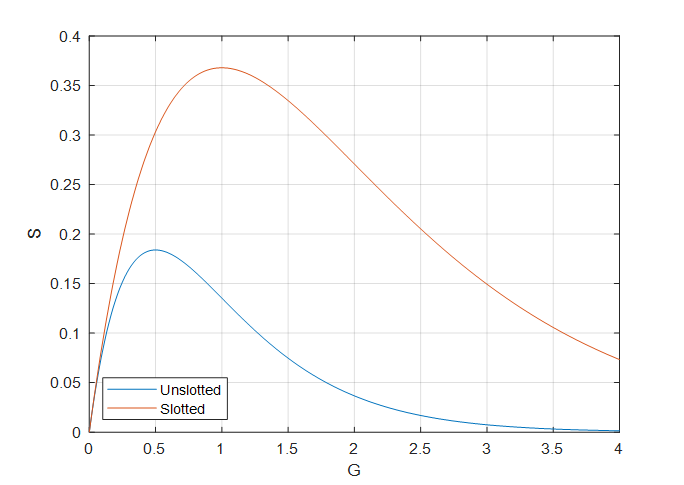
\includegraphics[width=15cm]{fig/RACH_ALOHA_throughput.png}
 \caption{The throughput of ALOHA system.}
 \label{fig:RACH_ALOHA_throughput}
\end{figure}

Fig. \ref{fig:RACH_ALOHA_throughput} is the throughput of ALOHA system. For unslotted system, $G = 0.5$ has the largest throughput $S \approx 0.1839 $, and for slotted system, $G = 1$ has the largest throughput $S \approx 0.3679$.

Based on the conventional ALOHA scheme, several random access protocols were developed \cite{alohaspread2005} \cite{massey1981collision} \cite{slottedalohathroughput} \cite{unslottedCDMA}. Most of them used more channel resources to avoid collisions, e.g.,  Spread-ALOHA will increase the spectrum usages, carrier sensing multiple access (CSMA) will increase the carrier usages, etc. Some researches are to resolve collision by contention tree or contention stack based on ALOHA re-transmission. However, there are more device connections, fewer channel resources, and low latency in modern communication systems. We introduced a novel RA scheme to resolve the collisions without additional channel resources, which is a similar GDMA concept.

\section{System Model}



\subsection{OFDM-GDMA system}

The proposed scheme can be applied to an orthogonal-frequency division multiplexing (OFDM) system.   For each $i \in \{0, 1, ...,N/(mQ)-1\}$, the subblock $[x_u(iQ+1), ..., x_u((i+1)Q)]$ is input into the $Q$-point inverse fast Fourier transform (IFFT) device to obtain the time domain signal. A cyclic prefix (CP) is inserted so as to avoid inter-symbol interference (ISI) and inter-carrier interference (ICI). On the receiver side, following CP removal and the $Q$-point FFT process, the frequency domain signal is then sent to the multi-level receiver.  Let $H_u(j)$ be the channel gain between user-$u$ and the receiver over the $j$-th sub-channel for $j \in \{1,...,Q\}$.  For the frequency domain signal, the component in the $j$-th sub-channel is
\begin{equation}
 r(iQ+j) = \sum_{u=1}^{U} H_u(j) x_{u}(iQ+j) + W(iQ+j),
\end{equation}
where $W(iQ+j)$ is the AWGN. The clustering-based channel estimation is performed for each of the sub-channels separately.

\subsection{Doppler-effect and unknown timing drift}
\label{s:Doppler-effect and unknown timing drift}

\begin{figure}[t!]
 \centering
 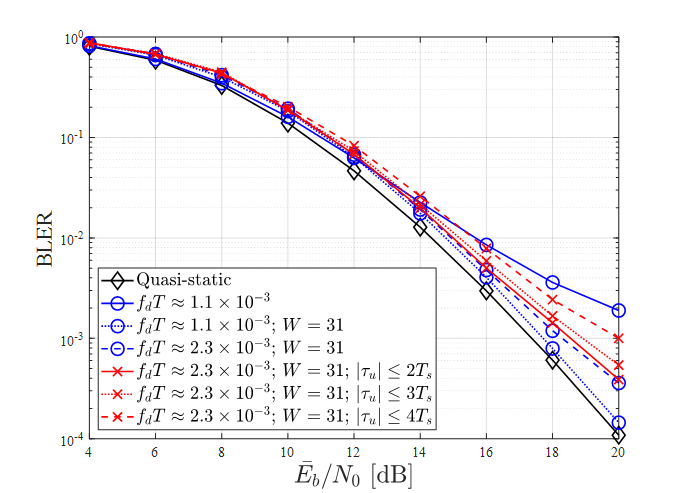
\includegraphics[width=15cm]{fig/OFDM_GDMA_doppler_timedrift.png}
 \caption{BLER performances for a (1008,504) LDPC-coded OFDM-GDMA
system where U = 2 users over frequency-selective Rayleigh fading channels.}
 \label{fig:OFDM_GDMA_doppler_timedrift}
\end{figure}

We now consider applying the proposed scheme to time-variant channels.  The basic settings are those depicted in Fig.~\ref{fig:OFDM_GDMA_doppler_timedrift} with $U$ = 2 and GMM.  To trace the traversal of channel gains which vary with time, we employ a sliding-window approach in the estimation process and the size of the window is set to $W$.  Consider the $i$-th windowing operation for $i \in \{0, 1, ..., n-W\}$.  The estimator only takes the received symbols $[r(iQ+j),...,r((i+W-1)Q+j)]$ as input samples for the clustering in order to estimate the channel gain $\hat{h}_{i,j}$ at symbol time $i + \lfloor W/2 \rfloor$ over the $j$-th sub-channel. The estimate $\hat{h}_{i,j}$ at $i = 0, 1, ..., \lfloor W/2 \rfloor-1$ is set to $\hat{h}_{\lfloor W/2 \rfloor,j}$.
Moreover,  $\hat{h}_{i,j}$ at $i \in \{n-\lfloor W/2 \rfloor-1, ..., n-W\}$ is set to $\hat{h}_{n-\lfloor W/2 \lfloor,j}$.
In the simulations shown in Fig.~\ref{fig:OFDM_GDMA_doppler_timedrift}, the maximum Doppler frequency $f_d$ is normalized using the period of an OFDM symbol $T$ which does not include CP. For $f_dT \approx 1.1 \times 10^{-3}$, the proposed estimation scheme
using the sliding window procedure with $W$ = 31 can achieve a BLER very close to that of the quasi-static case.  If windowing is not used, the BLER performance is significantly degraded for $f_dT \approx 1.1 \times 10^{-3}$ as indicated by the solid line with square symbols.

  We further consider an OFDM-GDMA system that has imperfect synchronization.  The simulation results are also provided in Fig.~\ref{fig:OFDM_GDMA_doppler_timedrift}.  Assume that user $u$ out of the $U$=2 users transmits a signal that is independent of the other user and has a uniformly distributed timing offset $\tau_u$ which is unknown to the receiver. Both the transmitting and receiving filters are square root raised cosine filters with a roll-off factor $\beta=0.22$.  In each transmitter, the  subblock $[x_u(iQ+1), ..., x_u((i+1)Q)]$ is up-sampled by a factor of 4, a $4Q$-point IFFT is used, and a cyclic suffix (CS) is added to prevent the interference from the other user.  By setting the CP length to $4T_s$ and the CS length to $4T_s$, we see that for $|\tau_u| \le 2T_s$, there is no performance loss when compared to the $|\tau_u| = 0$ case, where $T_s = \frac{T}{Q} = \frac{T}{16}$.
  
 

\subsection{Slotted RA OFDM-GDMA system}

In this system, all devices are synchronized before transmitting packets, e.g., RACH based system, and the length of each slot is OFDM symbol length. For the grant-based system, the receiver known the number of users. Multiple users can be detected by conventional GDMA. We can design a tolerance range, which can be designed by different cyclic prefix (CP) or cyclic suffix (CS) as section.\ref{s:Doppler-effect and unknown timing drift}. If the unknown drift of each device time is within the tolerance range, it can be solved. However, the wider tolerance range will waste more transmission. For the Grant-free system, the receiver does not know the number of users, and it can use the parity check of the LDPC code to determine which $U$ is most suitable for the current case as the paper\cite{hsu2020uplink}.


\subsection{Unslotted RA OFDM-GDMA system}

In this system, each device has not been synchronized with the receiver, and may be transmitted at any time, e.g., a RACH-free system. Unlike Slotted GDMA OFDM, we define the unit of GDMA is symbol length because the messages between each symbol are transmitted in parallel by different sub-carriers. If an OFDM symbol collides and the collision's time drift is within the tolerance range, it can be successfully resolved in this symbol. If the collision's time drift is outside the range, inter symbol interference(ISI) will be generated. Assume that $\tau_{1}$ is the transmission time of user-1 and $\tau_2$ is for user-2, and divide it into two case for discussions as fig.\ref{fig:RACH_unslotted_collision} from the perspective of user-1.

\begin{figure}[b!]
 \centering
 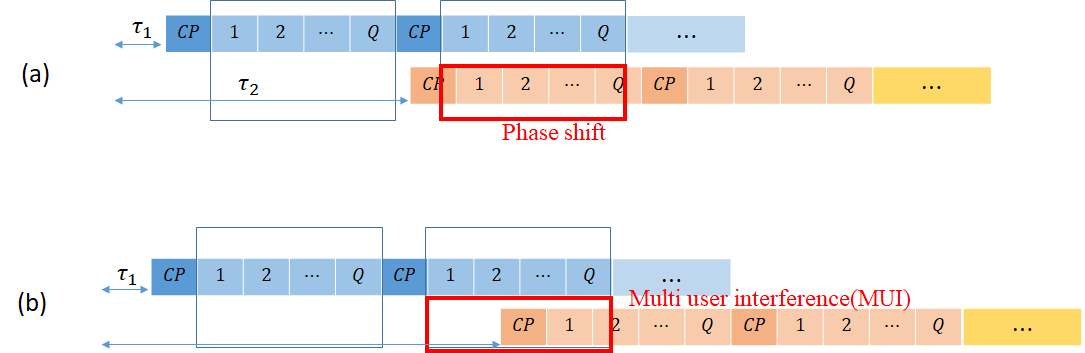
\includegraphics[width=15cm]{fig/RACH_unslotted_collision.png}
 \caption{(a) case 1 (b) case 2}
 \label{fig:RACH_unslotted_collision}
\end{figure}

Fig.\ref{fig:RACH_unslotted_collision}-(a) is the condition for $i \cdot N_s-\text{CP} < \tau_2 - \tau_ 1 < i \cdot N_s$, where $i=0, 1,  \cdots , N/mQ, N_s = \text{CP} + Q$. For $j=0,1, \cdots ,i-1$, derive the user-1 messages directly by using APP detector, since the symbol of user-1 does not collide. For $j=i, \cdots N/mQ$, set $U=2$ to detect user-1 and user-2 messages by using GDMA detector, since the truncated OFDM symbols of user-2 still have complete symbol information, which is only a phase shift in frequency domain.
   
Fig\ref{fig:RACH_unslotted_collision}-(b) is the condition on $ i \cdot N_s < \tau_2 - \tau_1 < (i+1) \cdot N_s + \text{CP}$, where $i=0, 1, \cdots,N/mQ$. If $j=0, \cdots, i-1$, derive the user-1 messages directly by using APP detector, since the symbol of user-1 does not collide.  If $j=i, \cdots N/mQ$, set user $U=2$ for detecting two user. However, the trancated symbol only contain complete user-1 OFDM symbol, e.g., the user-2 symbol is imcomplete that will generate inter symbol interference(ISI). Hence, we also need consider the ISI variance for APP detector. $\sigma_w^2$ must be adjusted for detecting APPs more accurately and be expressed as $\sigma_w^2$ = ISI variance + AWGN variance. Since the ISI noise has different effect for different SNR received signal, we adjust $\sigma_w^2$ with SNR, which is expressed as
$\sigma_w^2 = {( \sigma_{AWGN} + \mu \cdot \sqrt{i} )}^2$
, where $i$ is the SNR(dB). In practical situation, we do not known the SNR(dB) information beforehand. In future work, we may use the preamble to estimate the SNR(dB) information for accurately estimating MUI.


\section{Preamble Synchronization}
\subsection{Preamble}

There are some widely used preamble sequences, zadoff-chu (ZC) sequence, Pseudorandom (PN) sequence, Gold sequence, etc. In this thesis, we used the zadoff-chu sequence \cite{zepernick2013pseudo}. Zadoff-Chu sequences are used in the 3GPP NR in Primary Synchronization Signal(PSS), random access preamble(PRACH), etc. 

The zadoff-chu sequence at position $n$ is given by
\begin{align}
x_u(n) = e^{-j \pi u n (n+1)}, 0 \leq n \leq N_{ZC}-1 \\
u \in \{ 1, \cdots, N_{ZC}-1 \}, \text{gcd} (N_{ZC},u) = 1
\end{align}

, where $u$ is the root index.

Zadoff-Chu sequences exhibit following useful property:
	
\begin{enumerate}[leftmargin=\leftmargin+\widthof{Prefix}]
\item[(1)] The amplitude of the sequences is constant, and the sequence is orthogonal to their cyclic shift.
\item[(2)]  They are periodic with period $N_{ZC}$ if $N_{ZC}$ is odd. $x_u (n+N_ZC )=x_u (n)$.
\item[(3)] If $N_{zc}$ is prime, the Discrete Fourier Transform of a Zadoff-Chu sequence is an another Zadoff-Chu sequence conjugated. $X_u [k]=x_{u}^{*} (\widetilde{u_k}) X_u [0]$, where $\widetilde{u_k}$ is the multiplicative inverse of $u$ modulo $N_{ZC}$.
\item[(4)] The auto correlation of a Zadoff-Chu sequence with a cyclically shifted version of itself is zero.
\item[(5)] The cross-correlation between two prime length Zadoff-Chu sequences, i.e. different values of $u, u=u_1, u=u_2$ is constant $\frac{1}{\sqrt{N_{ZC}}}$, provided that $u_1-u_2$ is the relatively prime to $N_{ZC}$.
\end{enumerate}

\subsection{Synchronization}

\begin{figure}[H]
 \centering
 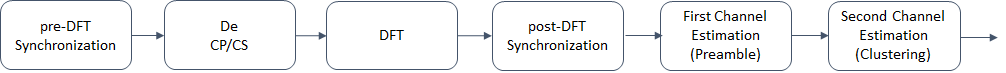
\includegraphics[width=17cm]{fig/synchronization_process.png}
 \caption{Synchronization and channel estimation process}
 \label{fig:Synchronization_process}
\end{figure}

Fig.\ref{fig:Synchronization_process} is the flow chart of synchronization and channel estimation, where pre-DFT synchronization is the coarse-timing estimation in the time domain, and post-DFT is the fine-timing estimation in the frequency domain. The channel estimation can also be divided into two steps, where first channel estimation only uses preamble to derive coarse gains. The second channel estimation use clustering to acquire fine gains based on the first channel estimation result.

\subsubsection{Coarse-timing estimate}

Coarse synchronization can be categorized into autocorrelation method and crosscorrelation method. For autocorrelation method, the transmitter adopts a repetitive structure. It only needs to calculate the autocorrelation of the received signal for estimating timing offset and frequency offset. For crosscorrelation method, the resultant approaches take advantage of cross-correlating received signals with receiver-generated preamble symbols. Derive estimated rough time offset by choosing the mean of timing metric trajectory peak.

In this thesis, we use the crosscorrelation method for implementation. Define the timing metric $c[n]$, and the crosscorrelation is expressed as

\begin{align}
c[n] = \frac{\sum_{i=0}^{N_{ZC}}(x_u[i]-\bar{x_u})^{*}(y[n+i]-\bar{y})}{\sqrt{\sum_{i=0}^{N_{ZC}}(x_u[i]-\bar{x_u})^{2}\sum_{i=0}^{N_{ZC}}(y[n+i]-\bar{y})^{2}}}
\end{align}

, where $y[i]$ is the received sample from time $i$, $\bar{y}$ is the mean of $y$, $\bar{x_u}$ is the mean of $x_u$,timing metric $|c[n]|<1$. If the timing metric is greater than threshold $\mu$ at time $\widehat{\theta}$, and estimate Time offset is $\widehat{\theta}$.

 In an additive white Gaussian noise (AWGN) channel, the coarse estimated time offset is at the exact timing point, but in multipath channels it would be shifted (delayed) due to the channel dispersion.

\subsubsection{Fine-timing estimate}

For deriving exact timing offset from a multipath channel, the fine time offset is necessary. Even under noiseless conditions, the timing estimate would be varying according to the time-varying channel. Accordingly, at different channel taps, the channel estimates would be delayed due to timing offset errors. If the delay in channel estimate can be found, the effect of the time-varying channel response on the timing estimation can be removed by simply delaying the coarse-timing estimation. In other words, the coarse timing estimate can be fine-tuned by adding the delay of the first actual channel tap. Define the fine time offset $\hat{\epsilon} =  \hat{\theta} - \theta$, where $\theta$ is the exact timing offset. For finding the delay of the first actual channel tap \cite{minn2003robust}, firstly, the strongest tap gain estimate $\hat{h}_{max}$ is found as $\hat{h}_{\text{max}} = \max_{l} \{ E_h(l) : l = 0, 1 , \cdots, K^{\dag}-K^{\prime} \} $. Then, the delay estimate of the first actual channel tap $\hat{\epsilon}$ is given by

\begin{align}
\hat{\epsilon} = \text{arg} \max_l \{ E_h(l) : l=0,1, \cdots,  K^{\dag}-K^{\prime} \}
\end{align}

where 

\begin{equation}
E_h(j)=
\left \{
\begin{array}{lr}
            \sum_{k=0}^{K^{\prime}-1} |\hat{h}_{l+k}|^2 &, \text{if} \  |\hat{h}_l| > \mu \cdot |\hat{h}_{\text{max}}|    \\
            0 &, \text{otherwise.} 
\end{array} \right.
\end{equation}

$E_h(l)$ is the channel energy estimation contained in a length-$K^{\prime}$ window starts from the tap $l$ with the condition that the channel energy estimate of the tap should be greater than threshold $\mu$. 

\section{Hybrid Channel Estimation}

Once obtaining the fine time offset $\hat{\epsilon}$, we can find the first tap of time-domain channel gains $\hat{h}[k]$ and derive the frequency domain channel gains $\hat{H}[k]$ directly by equ.\ref{equ:first_channel_estimation}.

\begin{align}
\label{equ:first_channel_estimation}
 & \hat{H}[k] = \frac{r[k]}{S[k]} e^{\frac{j2 \pi k\hat{\epsilon}}{N}}, k = 1,\cdots,N_{ZC} 
\\
 & \hat{h}[k] =  \text{IDFT}_{N_{ZC}} ( \hat{H[k]} ), k = 1,\cdots,N_{ZC} 
\end{align}

where $N_{ZC}$ is the preamble length and $S[k]; k=1, \cdots , N_{ZC}$ are the frequency domain preambles.


If preamble length $N_{ZC}$ is different from sub-carrier size $Q$, the estimated channel gains $\hat{H}[k]$ are also distinguished from sub-carrier channel gains $\tilde{H}$ which can be derived as 

\begin{align}
\tilde{H}[k] =  \text{FFT}_{Q} ( \hat{h[k]} ), k = 1,\cdots,Q 
\end{align}
,where the length of $\hat{h[k]}$ is $N_{ZC}$. It is only need the first $Q$ bits to derive sub-carrier channel gains $\tilde{H}$. 

Define $\tilde{H}[k]$ as first channel estimated gains and $\breve{H}[k]$ as second channel estimated gains. In chapter 3, we introduce several clustering algorithms for channel estimation. Hence, we use the clustering algorithm for estimating gains more accurately, which utensil $\tilde{H}[k]$ as the initial centroids. Fig.~\ref{fig:RACH_mse} is the MSE performance of first and second channel estimation, and the second estimation can achieve to CRLB, where we assume that perfect timing estimation.

\begin{figure}[t!]
 \centering
 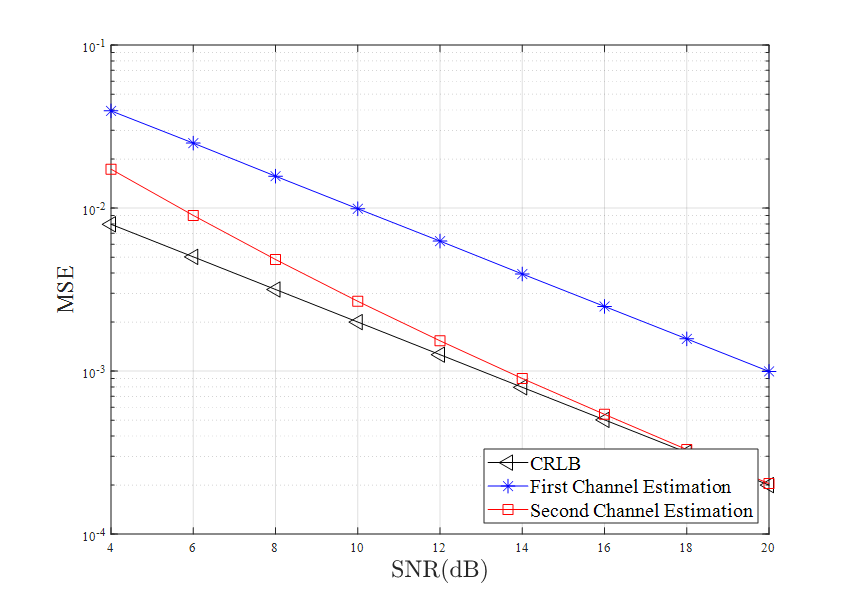
\includegraphics[width=15cm]{fig/RACH_mse.png}
 \caption{MSE comparison of first and second channel estimation}
 \label{fig:RACH_mse}
\end{figure}

\section{Simulation}

In following simulation, each packet has identical settings and contains a preamble sequence and OFDM sequence. In time domain, a packet length is expressed as : $\text{preamble length} + \text{OFDM symbol} \times \text{OFDM segment} = 71 + 20 \times 63 = 1331$, where the unit is $T_s$. Each packet is encoded by (1008,504) LDPC code. A OFDM symbol contain 4 CP and 16 IDFT sequence. A OFDM segment is 63. A preamble sequence is added to the packet header. The preamble sequence length is 71 , which contains 4 CP, 4 CS, and 63 zadoff-chu sequence with $N_{ZC}=63; u=25$.

Firstly, we discuss the case that no collision occurs in fig.\ref{fig:RACH_nocollision_case}. Define that the success rate is success $\frac{\text{transmitted packets}} {\text{total transmitted packets}}$. We found that the gap between timing perfect and timing estimation is larger than the gap between perfect CSI and second channel estimation. In our parameter setting, the synchronization success rate is more important than channel estimation. 

The situation in fig.\ref{fig:RACH_twocollision_case} is that two users will collide. Set $\tau_1$ as user-1 timing offset and $\tau_2$ as user-2 timing offset. Define that $|\tau_2 - \tau_1|$ is the uniform distribution with range from 0 to packet length. We found that the success rate based on second channel estimation will very close to perfect CSI. However, the time estimation success rate will also decrease obviously due to the preamble sequence collision. 

We assume that the start time of packets transmitted is a Poisson process having an average rate of $\lambda$ packets/s at receiver in 20 SNR(dB). Let $T_s$ denote the time duration of a packet. Then, the normalized channel traffic $G$, is defined as $G=\lambda \cdot T_s$ packets/duration. For a time duration, the probability of there being $k$ transmission is $\frac{G^k e^{-G}}{k!}$. We use the exponential distribution $f(x)=Ge^{-Gx}, x \ge 0 $ to simulate the time offset at receiver, e.g., the difference between $i$-packet and $i+1$-packet is $T_s \cdot f(x)$. To simulate precisely, we set simulation block  equal to $100 \cdot T_s$, and the exponential time offset is consequent in the block. The pseudo code of Poisson process is described as 

\begin{algorithm}[htb]
  \caption{ The pseudo code of Poisson process}
  \label{alg:Framwork}
  \begin{algorithmic}[1]
    \Require
      The time offset of each user is set as ${TN}_{u,i}$, where $u$-user has $TN_u$ packets, and $i = 1, \cdots, TN_u$.  $TO_{u,i}$ is the $u$-user $i$-packet time offset, which is a random number in the simulation block. 
    \Ensure
      Time offset differential of same user ${TO}_{u,i} - {TO}_{u,i-1}$ must be larger than a packet duration; \\
      Set $T_{\text{last}} = 0$ as last packet time \\
      Set $T_{\text{packet}}$ as packet duration \\
      Set $T_{\text{block}}$ as simulation block duration \\
      Set $f(x)=Ge^{-Gx}, x \ge 0$ as exponential distribution 
  	  \While { $T_{\text{last}} + T_{\text{packet}} \leq T_{\text{block}}$ }
      \State $T_{\text{last}} = T_{\text{last}} + f(x)$;
     
      \For{$u=1$; $u \leq U$; $u++$ }
      \If {$TN_u = 0 \parallel T_{\text{last}} - TO_{u,i} \geqslant T_{\text{packet}}$ }
      	\State ${TN}_{u,{TN_u}} = T_{\text{last}}$;
      	\State $TN_u = TN_u +1$ ;
      	\State break;
      \EndIf
      \EndFor
    \EndWhile \\
    \Return ${TN}_{u,i}$ and $TN_u$;
  \end{algorithmic}
\end{algorithm}


Fig.\ref{fig:ALOHA_system_simulation} is the throughput for simulated ALOHA system by above simulator,and we can find that it is equal to theory throughput in the simulator setting.



Firstly, we found that the Multi-User Interference (MUI) noise term influence greatly in high SNR. It take MUI noise as zero in fig.\ref{fig:RACH_poisson_case}, and take MUI noise as adapt variance in fig.\ref{fig:RACH_poisson_case2}, where the largest throughput $S \approx 0.4492 $ in fig.\ref{fig:RACH_poisson_case}, $S \approx 0.6088$ in fig.\ref{fig:RACH_poisson_case2}. Compare to unslotted ALOHA, the throughput of RA-OFDM-GDMA is raise obviously. For unslotted ALOHA, $G = 0.5$ has the largest throughput $S \approx 0.1839 $, and for RA-OFDM-GDMA, $G = 1.8$ has the largest throughput $S \approx 0.6088$ with perfect timing estimation and perfect CSI.
For timing estimation and channel estimation case, the largest throughput $S \approx 0.4107$ at $G=1.4$, which is still better than the slotted ALOHA theory.





\begin{figure}[t!]
 \centering
 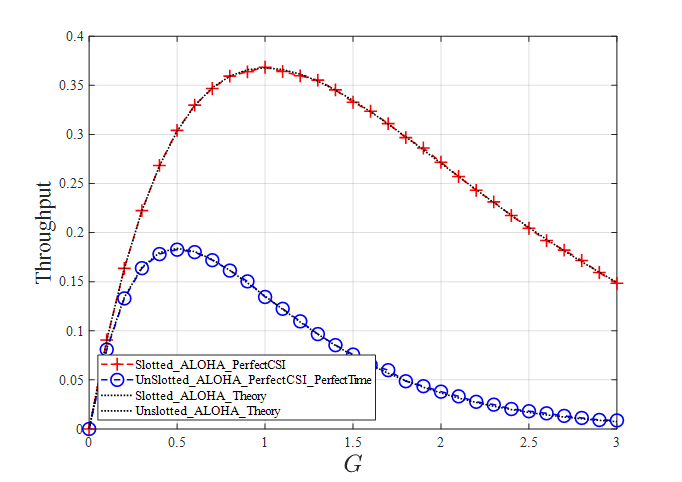
\includegraphics[width=15cm]{fig/RACH_ALOHA_throughput_simulation.png}
 \caption{ALOHA system simulation}
 \label{fig:ALOHA_system_simulation}
\end{figure}


\begin{figure}[t!]
 \centering
 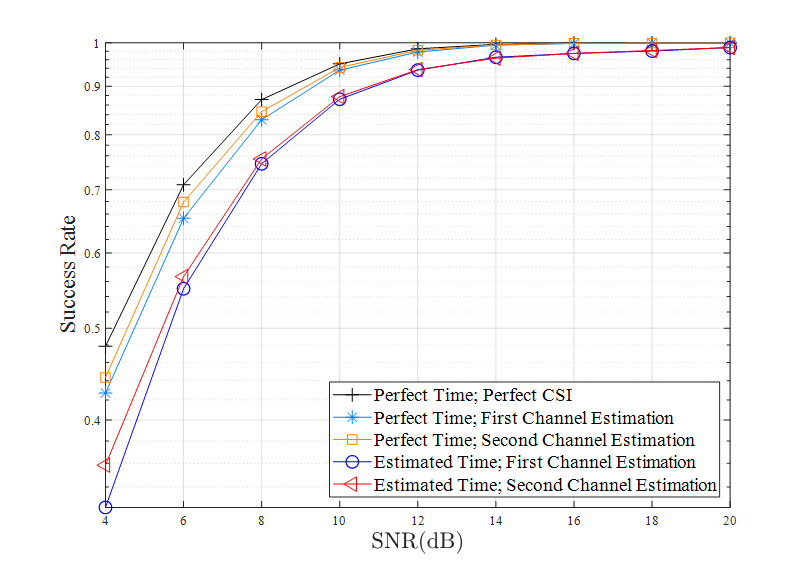
\includegraphics[width=15cm]{fig/RACH_nocollision_case.png}
 \caption{No user collision case}
 \label{fig:RACH_nocollision_case}
\end{figure}

\begin{figure}[b!]
 \centering
 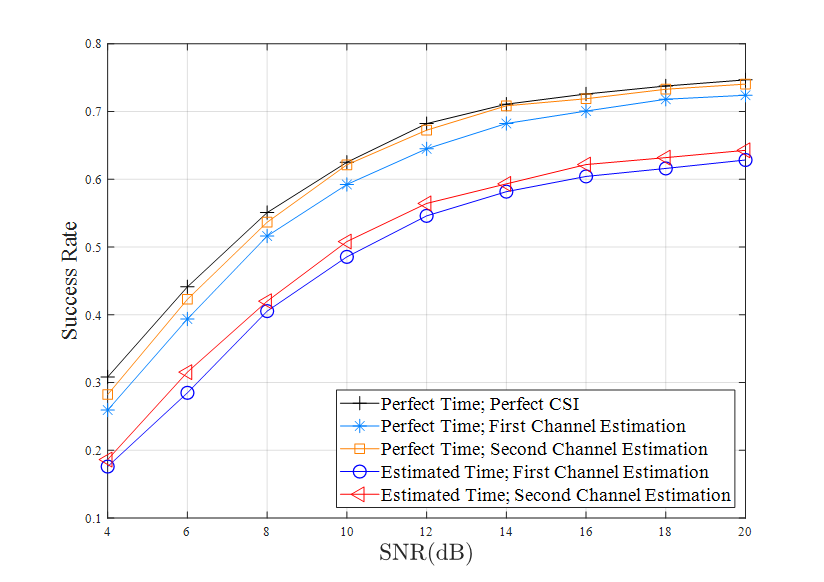
\includegraphics[width=15cm]{fig/RACH_twocollision_case.png}
 \caption{Two user collision case}
 \label{fig:RACH_twocollision_case}
\end{figure}

\begin{figure}[t!]
 \centering
 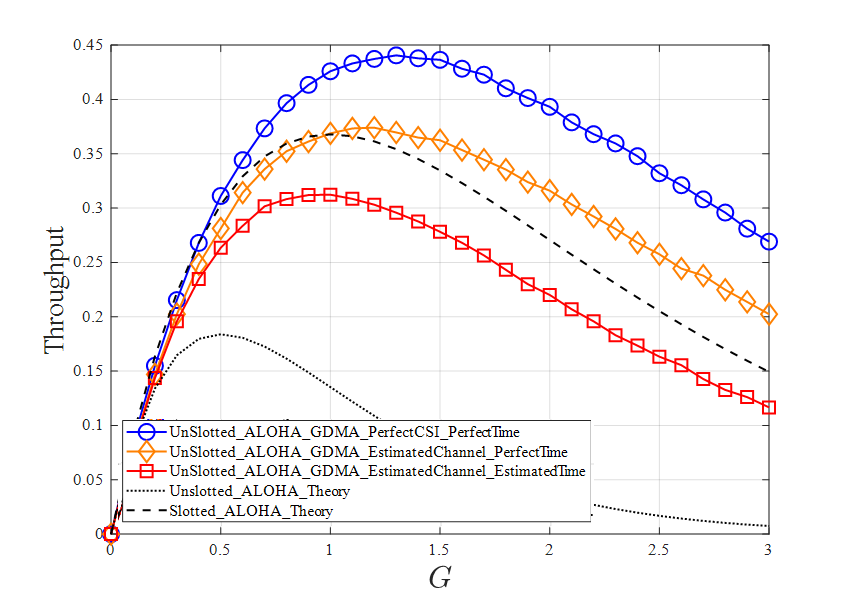
\includegraphics[width=14cm]{fig/RACH_poisson_case.png}
 \caption{The APP detector variance without considering MUI noise term in Poisson distribution collision case}
 \label{fig:RACH_poisson_case}
\end{figure}

\begin{figure}[b!]
 \centering
 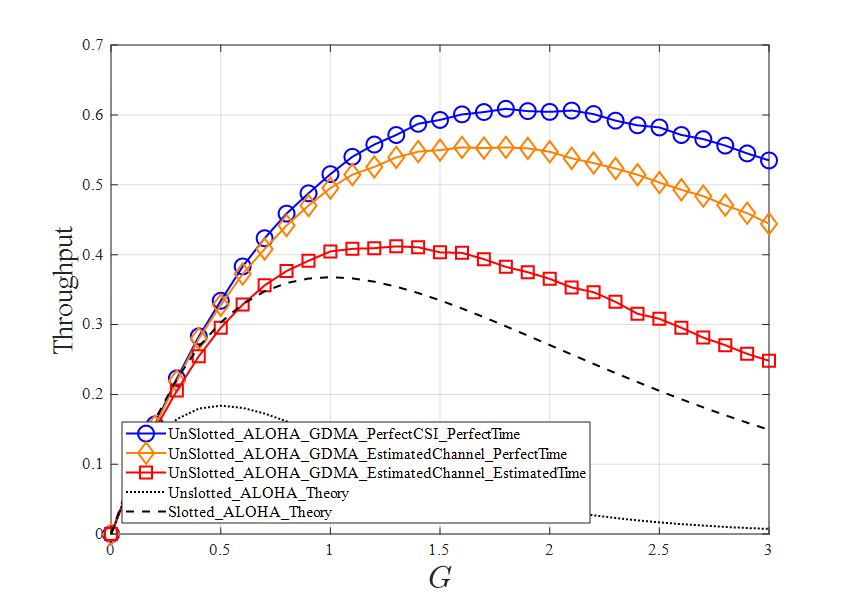
\includegraphics[width=14cm]{fig/RACH_poisson_case2.png}
 \caption{The APP detector variance without considering MUI noise term in Poisson distribution collision case}
 \label{fig:RACH_poisson_case2}
\end{figure}

